%=================================================================
% CSE 4345 — Big Data Analytics
% Week 6, Part 2: Seminal Research & Case Study
% Department of CSE, Premier University
%
% SEMINAL PAPERS:
%   Zaharia et al. (2010) — Spark: Cluster Computing with Working Sets
%   HotCloud 2010. (cited >5,000 times)
%
%   Zaharia et al. (2012) — Resilient Distributed Datasets: A
%   Fault-Tolerant Abstraction for In-Memory Cluster Computing.
%   NSDI 2012. (cited >13,000 times)
%
% CASE STUDY:
%   Databricks Daytona GraySort (2013) — 100 TB sorted in 23 min
%   on 206 EC2 instances; 3x faster than Hadoop on 3.5x fewer nodes
%=================================================================

\documentclass[aspectratio=169,10pt]{beamer}

%---------- Packages ----------
\usepackage[utf8]{inputenc}
\usepackage[T1]{fontenc}
\usepackage{booktabs}
\usepackage{xcolor}
\usepackage{tikz}
\usetikzlibrary{shapes.geometric, positioning, arrows.meta, decorations.pathreplacing}
\usepackage{amsmath}
\usepackage{graphicx}
\usepackage{multicol}
\usepackage{enumerate}
\usepackage{array}

%---------- Theme ----------
\usetheme{Madrid}

%---------- Premier University Color Identity ----------
\definecolor{PUNavy}{RGB}{10,36,99}
\definecolor{PUGold}{RGB}{197,151,37}
\definecolor{PULightBlue}{RGB}{210,228,255}
\definecolor{PUTeal}{RGB}{0,100,100}
\definecolor{PUGray}{RGB}{90,90,90}
\definecolor{PURed}{RGB}{160,30,30}
\definecolor{PUGreen}{RGB}{30,120,60}
\definecolor{PUPurple}{RGB}{90,30,120}
\definecolor{PUOrange}{RGB}{190,90,20}

\setbeamercolor{palette primary}{bg=PUNavy, fg=white}
\setbeamercolor{palette secondary}{bg=PUNavy!85, fg=white}
\setbeamercolor{palette tertiary}{bg=PUNavy!70, fg=white}
\setbeamercolor{palette quaternary}{bg=PUNavy, fg=white}
\setbeamercolor{structure}{fg=PUNavy}
\setbeamercolor{title}{bg=PUNavy, fg=PUGold}
\setbeamercolor{subtitle}{fg=white}
\setbeamercolor{frametitle}{bg=PUNavy, fg=PUGold}
\setbeamercolor{alerted text}{fg=PUGold!85!black}
\setbeamercolor{block title}{bg=PUNavy, fg=white}
\setbeamercolor{block body}{bg=PULightBlue!45}
\setbeamercolor{block title alerted}{bg=PUGold!80!black, fg=white}
\setbeamercolor{block body alerted}{bg=PUGold!12}
\setbeamercolor{block title example}{bg=PUTeal, fg=white}
\setbeamercolor{block body example}{bg=PUTeal!10}
\setbeamercolor{section in toc}{fg=PUNavy}
\setbeamercolor{itemize item}{fg=PUGold!80!black}
\setbeamercolor{itemize subitem}{fg=PUNavy!70}

\setbeamertemplate{navigation symbols}{}
\setbeamertemplate{itemize item}{\scriptsize\raise1.5pt\hbox{\textbullet}}
\setbeamertemplate{itemize subitem}{\scriptsize\raise1pt\hbox{--}}

%---------- Section separator ----------
\AtBeginSection[]{
  \begin{frame}[plain]
    \vfill
    \centering
    \begin{beamercolorbox}[sep=12pt,center,shadow=true,rounded=true]{block title}
      \usebeamerfont{title}\insertsectionhead\par
    \end{beamercolorbox}
    \vfill
  \end{frame}
}

%---------- Helper: citation box ----------
\newenvironment{paperbox}[1]{%
  \setbeamercolor{block title}{bg=PUNavy!90,fg=PUGold}
  \setbeamercolor{block body}{bg=PUNavy!6}
  \begin{block}{#1}}{%
  \end{block}}

%---------- Custom footline ----------
\setbeamertemplate{footline}{
  \leavevmode\hbox{%
    \begin{beamercolorbox}[wd=.333\paperwidth,ht=2.25ex,dp=1ex,center]{palette primary}
      \usebeamerfont{author in head/foot}\insertshortauthor
    \end{beamercolorbox}%
    \begin{beamercolorbox}[wd=.334\paperwidth,ht=2.25ex,dp=1ex,center]{palette secondary}
      \usebeamerfont{title in head/foot}\insertshorttitle
    \end{beamercolorbox}%
    \begin{beamercolorbox}[wd=.333\paperwidth,ht=2.25ex,dp=1ex,right]{palette primary}
      \usebeamerfont{date in head/foot}
      \insertframenumber{} / \inserttotalframenumber\hspace*{2ex}
    \end{beamercolorbox}}%
  \vskip0pt%
}

%---------- Title metadata ----------
\title[CSE 4345 \textbar{} Week 6, Part 2]{CSE 4345: Big Data Analytics}
\subtitle{Week 6, Part 2 \textemdash\ Seminal Research \& Case Study}
\author[Dept.\ of CSE]{Department of Computer Science \& Engineering\\[4pt]
       \small Premier University, Chittagong}
\institute{}
\date{Semester 2026}

%=================================================================
\begin{document}
%=================================================================

%----------------------------------------------------------------
% TITLE SLIDE
%----------------------------------------------------------------
\begin{frame}
  \titlepage
\end{frame}

%----------------------------------------------------------------
% PART 2 OVERVIEW
%----------------------------------------------------------------
\begin{frame}{Part 2 Overview — Week 6}
  \begin{columns}[T]
    \column{0.47\textwidth}
      \begin{block}{Today's Agenda}
        \tableofcontents
      \end{block}

    \column{0.50\textwidth}
      \begin{exampleblock}{Seminal Papers Covered}
        \begin{enumerate}
          \item Zaharia, M., et al. (2010).
                \textit{Spark: Cluster Computing with Working Sets.}
                USENIX HotCloud 2010.
          \item Zaharia, M., et al. (2012).
                \textit{Resilient Distributed Datasets: A Fault-Tolerant
                Abstraction for In-Memory Cluster Computing.}
                USENIX NSDI 2012.
        \end{enumerate}
      \end{exampleblock}
      \vspace{6pt}
      \begin{alertblock}{Case Study}
        Databricks Daytona GraySort (2013): 100~TB sorted in
        \textbf{23 minutes} on 206 EC2 nodes — $3\times$ faster than
        Hadoop on $3.5\times$ fewer machines.
      \end{alertblock}
      \vspace{4pt}
      \begin{block}{CLO Addressed}
        \textbf{CLO3} — Explain in-memory distributed processing\\
        \textbf{PLO(b,c)}
      \end{block}
  \end{columns}
\end{frame}

%================================================================
\section{Paper 1 — Zaharia et al.\ (2010): Spark HotCloud}
%================================================================

%----------------------------------------------------------------
\begin{frame}{Research Landscape: In-Memory Cluster Computing}
  \begin{center}
  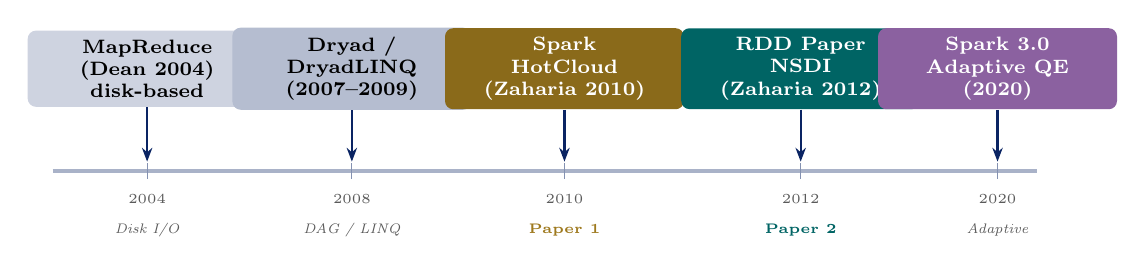
\begin{tikzpicture}[
      nbox/.style={rectangle, rounded corners=3pt, minimum width=3.0cm,
                   minimum height=0.9cm, text width=2.8cm, align=center,
                   font=\scriptsize\bfseries},
      arr/.style={-{Stealth[length=5pt]}, draw=PUNavy, thick}
    ]
    \draw[PUNavy!35, very thick] (0,0) -- (12.5,0);

    \node[nbox, fill=PUNavy!20]              (mr)   at (1.2, 1.3)
          {MapReduce\\(Dean 2004)\\disk-based};
    \node[nbox, fill=PUNavy!30]              (dryad)at (3.8, 1.3)
          {Dryad /\\DryadLINQ\\(2007--2009)};
    \node[nbox, fill=PUGold!70!black, text=white] (hc) at (6.5, 1.3)
          {Spark\\HotCloud\\(Zaharia 2010)};
    \node[nbox, fill=PUTeal, text=white]     (rdd)  at (9.5, 1.3)
          {RDD Paper\\NSDI\\(Zaharia 2012)};
    \node[nbox, fill=PUPurple!70, text=white](sp3)  at (12.0,1.3)
          {Spark 3.0\\Adaptive QE\\(2020)};

    \foreach \x/\y in {1.2/2004, 3.8/2008, 6.5/2010, 9.5/2012, 12.0/2020}{
      \draw[PUNavy!50] (\x,0.1) -- (\x,-0.1);
      \node[font=\tiny, text=PUGray] at (\x,-0.35) {\y};
    }

    \draw[arr] (mr)   -- (1.2,  0.12);
    \draw[arr] (dryad)-- (3.8,  0.12);
    \draw[arr] (hc)   -- (6.5,  0.12);
    \draw[arr] (rdd)  -- (9.5,  0.12);
    \draw[arr] (sp3)  -- (12.0, 0.12);

    \node[font=\tiny\itshape, text=PUGray]           at (1.2,  -0.75) {Disk I/O};
    \node[font=\tiny\itshape, text=PUGray]           at (3.8,  -0.75) {DAG / LINQ};
    \node[font=\tiny\bfseries, text=PUGold!80!black] at (6.5,  -0.75) {Paper 1};
    \node[font=\tiny\bfseries, text=PUTeal]          at (9.5,  -0.75) {Paper 2};
    \node[font=\tiny\itshape, text=PUGray]           at (12.0, -0.75) {Adaptive};
  \end{tikzpicture}
  \end{center}
  \vspace{4pt}
  \begin{alertblock}{The Fundamental Problem with MapReduce}
    Machine learning and graph algorithms are \textbf{iterative}: each
    iteration reads the output of the previous one.
    MapReduce writes every intermediate result to HDFS.
    For $k$ iterations: $k \times$ HDFS read + $k \times$ HDFS write.
    On spinning disk at 100~MB/s, 10 iterations over 100~GB costs
    \textbf{$\approx$3 hours of I/O alone}.
    Spark loads the dataset into RAM \emph{once} and iterates in memory.
  \end{alertblock}
\end{frame}

%----------------------------------------------------------------
\begin{frame}{Zaharia et al.\ (2010): HotCloud Publication Context}
  \begin{columns}[T]
    \column{0.53\textwidth}
      \begin{paperbox}{Full Citation}
        Zaharia, M., Chowdhury, M., Franklin, M.~J., Shenker, S., \&
        Stoica, I. (2010).
        \textbf{Spark: Cluster Computing with Working Sets.}
        In \textit{Proc.\ 2nd USENIX Workshop on Hot Topics in Cloud
        Computing (HotCloud '10)}. Boston, MA, USA.\\[5pt]
        \textbf{Venue:} USENIX HotCloud (workshop, short paper)\\
        \textbf{Cited by:} $>$5{,}000 (Google Scholar, 2024)\\
        \textbf{Authors:} Matei Zaharia (PhD student, UC Berkeley AMP Lab),
        co-advised by Scott Shenker \& Ion Stoica
      \end{paperbox}
      \vspace{5pt}
      \begin{exampleblock}{The Key Observation}
        Many real workloads operate on a \textbf{working set} —
        a dataset that is \emph{reused across multiple parallel operations}:
        \begin{itemize}\setlength\itemsep{0pt}
          \item Iterative ML (logistic regression, k-means): same dataset,
                many gradient steps
          \item Interactive analytics: analyst queries same table repeatedly
          \item Graph algorithms: same graph, many BFS/SSSP passes
        \end{itemize}
        MapReduce cannot cache a working set across jobs.
      \end{exampleblock}

    \column{0.44\textwidth}
      \begin{block}{Working Set vs.\ Streaming}
        \begin{center}
        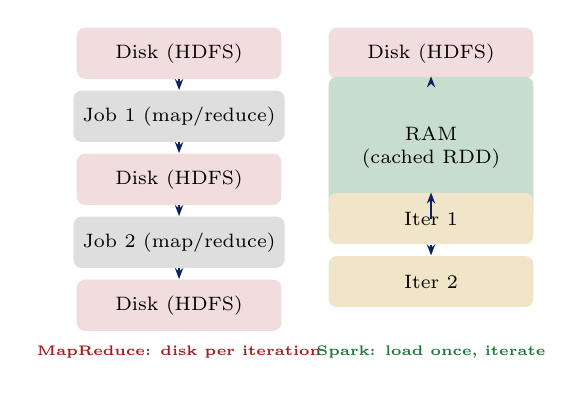
\begin{tikzpicture}[
            bx/.style={rectangle, rounded corners=3pt, minimum width=2.6cm,
                       minimum height=0.65cm, align=center, font=\scriptsize},
            arr/.style={-{Stealth[length=4pt]}, draw=PUNavy, thick}
          ]
          % MapReduce path
          \node[bx, fill=PURed!15]  (d1) at (0, 3.5) {Disk (HDFS)};
          \node[bx, fill=PUGray!20] (j1) at (0, 2.7) {Job 1 (map/reduce)};
          \node[bx, fill=PURed!15]  (d2) at (0, 1.9) {Disk (HDFS)};
          \node[bx, fill=PUGray!20] (j2) at (0, 1.1) {Job 2 (map/reduce)};
          \node[bx, fill=PURed!15]  (d3) at (0, 0.3) {Disk (HDFS)};
          \draw[arr] (d1)--(j1); \draw[arr] (j1)--(d2);
          \draw[arr] (d2)--(j2); \draw[arr] (j2)--(d3);
          \node[font=\tiny\bfseries, text=PURed] at (0,-0.3)
                {MapReduce: disk per iteration};

          % Spark path (right)
          \node[bx, fill=PURed!15]  (sd) at (3.2, 3.5) {Disk (HDFS)};
          \node[bx, fill=PUGreen!25, minimum height=1.8cm]
                (ram) at (3.2, 2.3) {RAM\\(cached RDD)};
          \node[bx, fill=PUGold!25] (i1) at (3.2, 1.4) {Iter 1};
          \node[bx, fill=PUGold!25] (i2) at (3.2, 0.6) {Iter 2};
          \draw[arr] (sd)--(ram);
          \draw[arr] (ram)--(i1); \draw[arr] (i1)--(i2);
          \node[font=\tiny\bfseries, text=PUGreen] at (3.2,-0.3)
                {Spark: load once, iterate};
        \end{tikzpicture}
        \end{center}
      \end{block}
  \end{columns}
\end{frame}

%================================================================
\section{Paper 2 — Zaharia et al.\ (2012): RDDs at NSDI}
%================================================================

%----------------------------------------------------------------
\begin{frame}{Zaharia et al.\ (2012): NSDI Publication Context}
  \begin{columns}[T]
    \column{0.53\textwidth}
      \begin{paperbox}{Full Citation}
        Zaharia, M., Chowdhury, M., Das, T., Dave, A., Ma, J.,
        McCauley, M., Franklin, M.~J., Shenker, S., \& Stoica, I.
        (2012).
        \textbf{Resilient Distributed Datasets: A Fault-Tolerant
        Abstraction for In-Memory Cluster Computing.}
        In \textit{Proc.\ 9th USENIX Symposium on Networked Systems
        Design and Implementation (NSDI '12)}, pp.~15--28.
        San Jose, CA, USA.\\[5pt]
        \textbf{Venue:} USENIX NSDI — Rank A* (CORE), top systems venue\\
        \textbf{Cited by:} $>$13{,}000 (Google Scholar, 2024)\\
        \textbf{Best Paper Award:} NSDI 2012
      \end{paperbox}
      \vspace{5pt}
      \begin{exampleblock}{From Workshop to Full Paper}
        The 2010 HotCloud paper was a \textbf{4-page proof-of-concept}.
        The 2012 NSDI paper introduced \textbf{RDDs} as a formal
        abstraction, provided a full implementation description,
        and presented rigorous benchmarks on real workloads.
        This is the paper that defined modern Spark.
      \end{exampleblock}

    \column{0.44\textwidth}
      \begin{block}{The RDD Definition}
        \begin{center}
        \large\color{PUNavy}
        \textit{``A \textbf{Resilient Distributed Dataset} is a read-only,
        partitioned collection of records that can be created through
        deterministic operations on data in stable storage or
        other RDDs.''}
        \end{center}
        \vspace{4pt}
        \scriptsize
        \begin{itemize}
          \item \textbf{Resilient}: lost partitions are recomputed
                from lineage, not replicated checkpoints
          \item \textbf{Distributed}: partitions spread across nodes
          \item \textbf{Dataset}: a collection of records,
                not a mutable key-value store
        \end{itemize}
      \end{block}
  \end{columns}
\end{frame}

%----------------------------------------------------------------
\begin{frame}{Technical Contribution 1 — RDD Lineage \& Fault Tolerance}
  \begin{columns}[T]
    \column{0.50\textwidth}
      \begin{block}{Lineage Graph: The Key Innovation}
        RDDs do \textbf{not replicate data} to tolerate failures.
        Instead, each RDD records a \textbf{lineage}:
        a log of the transformations that produced it.
        If a partition is lost, Spark re-executes only those
        transformations on the relevant input partitions.\\[5pt]
        \textbf{Two types of operations}:
        \begin{itemize}
          \item \textbf{Transformations} (lazy): \texttt{map},
                \texttt{filter}, \texttt{flatMap}, \texttt{groupByKey},
                \texttt{reduceByKey}, \texttt{join} — return a new RDD,
                do \emph{not} trigger computation
          \item \textbf{Actions} (eager): \texttt{count}, \texttt{collect},
                \texttt{reduce}, \texttt{saveAsTextFile} — trigger
                a DAG execution from root to output
        \end{itemize}
      \end{block}
      \vspace{4pt}
      \begin{exampleblock}{Lazy Evaluation Benefit}
        The driver builds the full DAG before execution begins.
        Catalyst (Spark SQL's optimiser) can reorder, fuse, or
        eliminate transformations \emph{before} a single task runs.
      \end{exampleblock}

    \column{0.47\textwidth}
      \begin{center}
      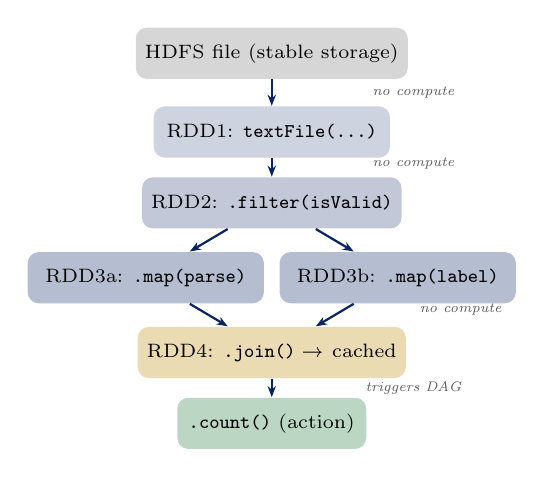
\begin{tikzpicture}[
          rd/.style={rectangle, rounded corners=4pt, minimum width=3.0cm,
                     minimum height=0.65cm, align=center, font=\scriptsize},
          arr/.style={-{Stealth[length=4pt]}, draw=PUNavy, thick},
          labl/.style={font=\tiny\itshape, text=PUGray}
        ]
        \node[rd, fill=PUGray!25]  (hdfs) at (0, 4.5)
              {HDFS file (stable storage)};
        \node[rd, fill=PUNavy!20]  (r1)   at (0, 3.5)
              {RDD1: \texttt{textFile(...)}};
        \node[rd, fill=PUNavy!25]  (r2)   at (0, 2.6)
              {RDD2: \texttt{.filter(isValid)}};
        \node[rd, fill=PUNavy!30]  (r3a)  at (-1.6, 1.65)
              {RDD3a: \texttt{.map(parse)}};
        \node[rd, fill=PUNavy!30]  (r3b)  at (1.6,  1.65)
              {RDD3b: \texttt{.map(label)}};
        \node[rd, fill=PUGold!35]  (r4)   at (0, 0.7)
              {RDD4: \texttt{.join()} \textrightarrow{} cached};
        \node[rd, fill=PUGreen!30, minimum width=2.4cm]
              (act)  at (0, -0.2) {\texttt{.count()} (action)};

        \draw[arr] (hdfs)--(r1);
        \draw[arr] (r1)  --(r2);
        \draw[arr] (r2)  --(r3a);
        \draw[arr] (r2)  --(r3b);
        \draw[arr] (r3a) --(r4);
        \draw[arr] (r3b) --(r4);
        \draw[arr] (r4)  --(act);

        \node[labl] at (1.8, 4.0)  {no compute};
        \node[labl] at (1.8, 3.1)  {no compute};
        \node[labl] at (2.4, 1.25) {no compute};
        \node[labl] at (1.8, 0.25) {triggers DAG};
      \end{tikzpicture}
      \end{center}
  \end{columns}
\end{frame}

%----------------------------------------------------------------
\begin{frame}{Technical Contribution 2 — Narrow vs.\ Wide Dependencies}
  \begin{columns}[T]
    \column{0.50\textwidth}
      \begin{block}{Dependency Classification}
        \textbf{Narrow dependency}: each parent partition contributes
        to \emph{at most one} child partition.
        \begin{itemize}
          \item Examples: \texttt{map}, \texttt{filter}, \texttt{union}
          \item No data shuffle required
          \item Lost partition recomputed from \textbf{one} parent partition
          \item Pipelined within a single \textbf{Stage} (no barrier)
        \end{itemize}
        \vspace{4pt}
        \textbf{Wide dependency}: each parent partition may contribute
        to \emph{multiple} child partitions.
        \begin{itemize}
          \item Examples: \texttt{groupByKey}, \texttt{reduceByKey},
                \texttt{sortByKey}, \texttt{join} (on un-partitioned RDDs)
          \item Requires a \textbf{shuffle} — network-intensive barrier
          \item Marks a Stage boundary in the DAG
          \item Lost partition requires re-computing \emph{all} parent partitions
        \end{itemize}
      \end{block}

    \column{0.47\textwidth}
      \begin{center}
      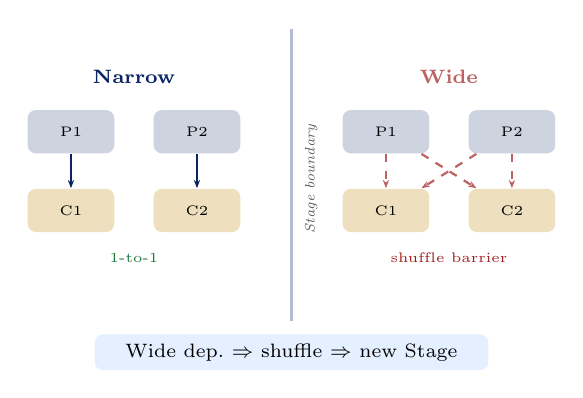
\begin{tikzpicture}[
          pt/.style={rectangle, rounded corners=3pt, minimum width=1.1cm,
                     minimum height=0.55cm, align=center, font=\tiny},
          arr/.style={-{Stealth[length=3pt]}, draw=PUNavy, thick},
          warr/.style={-{Stealth[length=3pt]}, draw=PURed!70, thick, dashed}
        ]
        % Narrow
        \node[font=\scriptsize\bfseries, text=PUNavy] at (-2.0, 3.9) {Narrow};
        \node[pt, fill=PUNavy!20] (np1) at (-2.8, 3.2) {P1};
        \node[pt, fill=PUNavy!20] (np2) at (-1.2, 3.2) {P2};
        \node[pt, fill=PUGold!30] (nc1) at (-2.8, 2.2) {C1};
        \node[pt, fill=PUGold!30] (nc2) at (-1.2, 2.2) {C2};
        \draw[arr] (np1)--(nc1);
        \draw[arr] (np2)--(nc2);
        \node[font=\tiny, text=PUGreen] at (-2.0, 1.6) {1-to-1};

        % Wide
        \node[font=\scriptsize\bfseries, text=PURed!70] at (2.0, 3.9) {Wide};
        \node[pt, fill=PUNavy!20] (wp1) at (1.2, 3.2) {P1};
        \node[pt, fill=PUNavy!20] (wp2) at (2.8, 3.2) {P2};
        \node[pt, fill=PUGold!30] (wc1) at (1.2, 2.2) {C1};
        \node[pt, fill=PUGold!30] (wc2) at (2.8, 2.2) {C2};
        \draw[warr] (wp1)--(wc1);
        \draw[warr] (wp1)--(wc2);
        \draw[warr] (wp2)--(wc1);
        \draw[warr] (wp2)--(wc2);
        \node[font=\tiny, text=PURed] at (2.0, 1.6) {shuffle barrier};

        % Stage boundary annotation
        \draw[PUNavy!30, very thick] (0, 0.8) -- (0, 4.5);
        \node[font=\tiny\itshape, text=PUGray, rotate=90] at (0.25, 2.6)
              {Stage boundary};

        % Implication box
        \node[rectangle, fill=PULightBlue!60, rounded corners=3pt,
              minimum width=5.0cm, align=center, font=\scriptsize]
              at (0, 0.4)
              {Wide dep.\ $\Rightarrow$ shuffle $\Rightarrow$ new Stage};
      \end{tikzpicture}
      \end{center}
  \end{columns}
\end{frame}

%----------------------------------------------------------------
\begin{frame}{Technical Contribution 3 — Persistence \& Partitioning}
  \begin{columns}[T]
    \column{0.50\textwidth}
      \begin{block}{Persistence Levels (from the paper)}
        \renewcommand{\arraystretch}{1.25}
        \begin{tabular}{@{}lp{5.0cm}@{}}
          \toprule
          \textbf{StorageLevel} & \textbf{Meaning} \\
          \midrule
          \texttt{MEMORY\_ONLY}      & JVM heap; spill re-computes \\
          \texttt{MEMORY\_AND\_DISK} & Heap; overflow to local disk \\
          \texttt{DISK\_ONLY}        & Local disk; slower reuse \\
          \texttt{MEMORY\_ONLY\_SER} & Kryo-serialised bytes in heap;
                                       smaller but slower \\
          \texttt{OFF\_HEAP}         & Native memory (Unsafe);
                                       avoids GC pressure \\
          \bottomrule
        \end{tabular}
      \end{block}
      \vspace{5pt}
      \begin{alertblock}{When to Cache?}
        Cache an RDD if it is \textbf{reused in $>$1 action}
        (iterative ML, interactive queries).
        Caching single-use RDDs wastes RAM and triggers eviction
        of other cached data (LRU eviction policy).
      \end{alertblock}

    \column{0.47\textwidth}
      \begin{block}{Partitioning for Key-Value RDDs}
        \begin{itemize}
          \item \textbf{Hash partitioner} (default):
                \texttt{key.hashCode() \% numPartitions}\\
                Uniform for random keys; can hot-spot on skewed data
          \item \textbf{Range partitioner}:
                samples key distribution, assigns ranges to partitions;
                used by \texttt{sortByKey()}
          \item \textbf{Custom partitioner}:
                user-supplied; co-partition two RDDs on the same key
                to eliminate shuffle on join
        \end{itemize}
      \end{block}
      \vspace{5pt}
      \begin{exampleblock}{Impact: Benchmark Results (RDD paper)}
        \textbf{Logistic regression} (10 iterations):
        \begin{itemize}
          \item Hadoop MapReduce: 127 s/iteration (disk)
          \item Spark (MEMORY\_ONLY): \textbf{0.96 s/iteration}
          \item Speedup: $\mathbf{132\times}$
        \end{itemize}
        \textbf{K-means clustering} (10 iterations):
        Hadoop 150~s vs.\ Spark 5~s = $\mathbf{30\times}$
      \end{exampleblock}
  \end{columns}
\end{frame}

%----------------------------------------------------------------
\begin{frame}{Impact Today — Zaharia et al.\ (2010, 2012)}
  \begin{columns}[T]
    \column{0.50\textwidth}
      \begin{block}{What Spark Built on the RDD Foundation}
        \begin{itemize}
          \item \textbf{Spark SQL / DataFrames} (2014):
                RDDs wrapped in a typed columnar schema;
                \textbf{Catalyst optimizer} rewrites logical plans;
                \textbf{Tungsten} generates JVM bytecode for execution
          \item \textbf{Spark Streaming / Structured Streaming} (2013/2016):
                micro-batch or continuous processing via DStreams
                (RDDs) and then DataStreamReader (DataFrames)
          \item \textbf{MLlib / ML Pipelines} (2014):
                iterative ML on cached DataFrames; Pipeline API
                mirrors scikit-learn's \texttt{fit}/\texttt{transform}
          \item \textbf{GraphX} (2014): RDD-backed property graphs
                for PageRank, label propagation, connected components
          \item \textbf{Delta Lake / Iceberg integration} (2019+):
                Spark is the primary compute engine for ACID
                lakehouse architectures
        \end{itemize}
      \end{block}

    \column{0.47\textwidth}
      \begin{exampleblock}{Stanford CS246 / MIT 6.830 Perspective}
        \begin{itemize}
          \item Stanford CS246 uses Spark as the reference platform
                for \textbf{graph mining} (PageRank via
                \texttt{GraphX}) and \textbf{recommendation systems}
                (ALS via MLlib); the RDD lineage model is presented
                as an instance of \textbf{dataflow programming}
          \item MIT 6.830 benchmarks Spark SQL vs.\ MonetDB
                (column store) on TPC-H: Spark SQL is within
                $2\times$ on analytical queries thanks to Catalyst
                predicate pushdown — despite being a general engine
          \item CMU 15-721 covers Tungsten's \textbf{whole-stage
                code generation} as a JIT compiler applied to
                relational operators — a modern take on query compilation
        \end{itemize}
      \end{exampleblock}
      \vspace{4pt}
      \begin{alertblock}{CLO3 Connection}
        RDDs + Catalyst + Tungsten directly address CLO3:
        \emph{how} Spark explains and optimises distributed
        in-memory computation.
      \end{alertblock}
  \end{columns}
\end{frame}

%================================================================
\section{Case Study — Databricks Daytona GraySort (2013)}
%================================================================

%----------------------------------------------------------------
\begin{frame}{The GraySort Benchmark}
  \begin{columns}[T]
    \column{0.52\textwidth}
      \begin{block}{What is Daytona GraySort?}
        GraySort (named after Jim Gray, Turing Award 1998) is the
        \textbf{world-record sorting competition} for large-scale
        data systems.  Two categories:
        \begin{itemize}
          \item \textbf{Daytona}: real-world rules — commodity hardware,
                standard sort record format (100-byte records,
                10-byte key), fault tolerance required, no code
                specialisation; the prestigious category
          \item \textbf{Indy}: custom hardware / software optimisations
                allowed
        \end{itemize}
        \textbf{Benchmark dataset}: 100~TB of random 100-byte records
        ($10^{12}$ records).\\[4pt]
        \textbf{Metric}: wall-clock time to sort, verify, and write output.
      \end{block}

    \column{0.45\textwidth}
      \begin{alertblock}{Previous Record (Yahoo!, 2009)}
        Yahoo!\ sorted 100~TB on a \textbf{3{,}800-node Hadoop
        MapReduce} cluster in \textbf{173 minutes}.
        In 2012, a team at Yahoo!\ improved the Hadoop record to
        \textbf{72 minutes} using 2{,}100 nodes.\\[6pt]
        Key bottleneck: MapReduce's sort phase writes intermediate
        data to disk between the map and reduce stages —
        twice for each byte (spill + merge).
        At 100~TB, this is $\approx$200~TB of additional disk I/O.
      \end{alertblock}
      \vspace{5pt}
      \begin{exampleblock}{Why Sort?}
        Sorting exercises every component of a distributed system:
        network bandwidth, disk I/O, CPU (comparison), memory,
        and distributed coordination.
        A faster sort implies a faster data platform in general.
      \end{exampleblock}
  \end{columns}
\end{frame}

%----------------------------------------------------------------
\begin{frame}{Databricks Result: 100 TB in 23 Minutes (November 2013)}
  \begin{columns}[T]
    \column{0.52\textwidth}
      \begin{block}{The Databricks Setup}
        \begin{itemize}
          \item \textbf{Cluster}: 206 EC2 \texttt{i2.8xlarge} instances
                on Amazon Web Services
          \item \textbf{Per node}: 32 vCPUs, 244~GB RAM, 8$\times$800~GB
                SSD (local ephemeral storage)
          \item \textbf{Total RAM}: $206 \times 244 = 50.3$~TB
          \item \textbf{Total SSD}: $206 \times 6.4 = 1.3$~PB
          \item \textbf{Network}: 10~Gbps per node
          \item \textbf{Input}: 100~TB of random 100-byte records
                stored in HDFS (3$\times$ replication = 300~TB on disk)
          \item \textbf{Spark version}: 0.8 (pre-DataFrame era)
        \end{itemize}
      \end{block}
      \vspace{4pt}
      \begin{block}{Result}
        \begin{center}
          \Large\color{PUNavy}
          \textbf{100 TB sorted in 23 minutes}
        \end{center}
        \begin{center}
          \small 4.27 TB/min throughput
        \end{center}
      \end{block}

    \column{0.45\textwidth}
      \begin{center}
      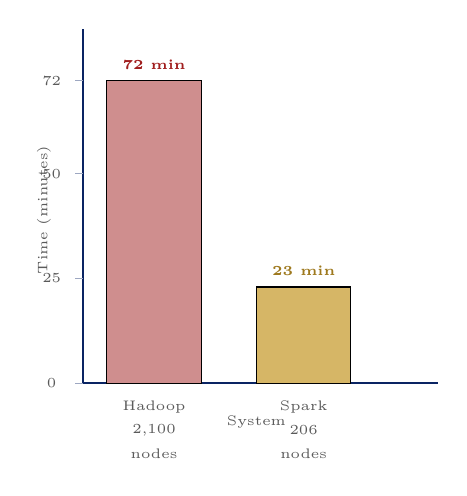
\begin{tikzpicture}[
          bar/.style={rectangle, minimum width=1.2cm, align=center,
                      font=\scriptsize\bfseries}
        ]
        % Axes
        \draw[PUNavy, thick] (0,0) -- (0,4.5);
        \draw[PUNavy, thick] (0,0) -- (4.5,0);
        \node[font=\tiny, text=PUGray, rotate=90] at (-0.5, 2.2)
              {Time (minutes)};
        \node[font=\tiny, text=PUGray] at (2.2, -0.5) {System};

        % Yahoo! 2012 Hadoop bar
        \draw[fill=PURed!50] (0.3, 0) rectangle (1.5, 3.84);
        \node[font=\tiny\bfseries, text=PURed] at (0.9, 4.05) {72 min};
        \node[font=\tiny, text=PUGray] at (0.9,-0.3) {Hadoop};
        \node[font=\tiny, text=PUGray] at (0.9,-0.6) {2,100};
        \node[font=\tiny, text=PUGray] at (0.9,-0.9) {nodes};

        % Databricks Spark bar
        \draw[fill=PUGold!70] (2.2, 0) rectangle (3.4, 1.22);
        \node[font=\tiny\bfseries, text=PUGold!80!black] at (2.8, 1.43) {23 min};
        \node[font=\tiny, text=PUGray] at (2.8,-0.3) {Spark};
        \node[font=\tiny, text=PUGray] at (2.8,-0.6) {206};
        \node[font=\tiny, text=PUGray] at (2.8,-0.9) {nodes};

        % Y-axis ticks
        \foreach \y/\lbl in {0/0, 1.33/25, 2.66/50, 3.84/72}{
          \draw[PUNavy!40] (-0.1,\y)--(0,\y);
          \node[font=\tiny, text=PUGray] at (-0.4,\y) {\lbl};
        }
      \end{tikzpicture}
      \end{center}
      \vspace{-4pt}
      \begin{alertblock}{\small Key Ratios}
        \begin{itemize}\setlength\itemsep{0pt}
          \item $3.1\times$ faster than Hadoop (72 min $\to$ 23 min)
          \item $10.2\times$ fewer nodes (2,100 $\to$ 206)
          \item \textbf{32$\times$ better efficiency} per node
        \end{itemize}
      \end{alertblock}
  \end{columns}
\end{frame}

%----------------------------------------------------------------
\begin{frame}{Why Spark Won: Technical Analysis}
  \begin{columns}[T]
    \column{0.52\textwidth}
      \begin{block}{What Made Spark Faster at GraySort?}
        \begin{enumerate}
          \item \textbf{Sort-based shuffle} (not hash-based):
                Spark's sort shuffle writes sorted runs to disk once,
                then merges — MapReduce's hash shuffle spills, merges,
                and re-reads multiple times.
                At 100~TB, this eliminates $\approx$120~TB of extra I/O.
          \item \textbf{SSD-aware I/O}: Databricks configured Spark to
                use all 8 SSDs as shuffle directories simultaneously —
                8$\times$ the sequential write bandwidth of one SSD.
          \item \textbf{Off-heap sort buffers}: Spark's \texttt{UnsafeShuffleWriter}
                uses sun.misc.Unsafe to sort records in native memory,
                bypassing JVM GC pauses during the sort phase.
          \item \textbf{Fewer stages}: the sort is a single wide
                transformation (\texttt{sortByKey}) — no intermediate
                HDFS writes between map and reduce.
        \end{enumerate}
      \end{block}

    \column{0.45\textwidth}
      \begin{exampleblock}{Databricks Production Spark ML (2014)}
        Beyond sorting, Databricks published results showing Spark
        MLlib outperforming Mahout (MapReduce-based ML):
        \begin{itemize}
          \item \textbf{Logistic regression} on 1~TB:
                Spark 2 min vs.\ Mahout 10+ hours
          \item \textbf{Collaborative filtering} (ALS) on Netflix data:
                Spark 35 min vs.\ MR implementation 10 hours
          \item The speedup comes \emph{primarily} from keeping the
                model and working set in RAM across iterations
        \end{itemize}
      \end{exampleblock}
      \vspace{4pt}
      \begin{block}{Long-Term Impact}
        The GraySort result generated enormous press coverage and
        directly drove Spark's adoption:
        Apache Spark went from 200 GitHub stars in 2013 to
        $>$36{,}000 by 2020;
        Databricks raised \$150M Series~B within 6 months of the record.
      \end{block}
  \end{columns}
\end{frame}

%----------------------------------------------------------------
\begin{frame}{Lessons Learned \& Discussion Questions}
  \begin{columns}[T]
    \column{0.52\textwidth}
      \begin{block}{Key Lessons from Spark's Rise}
        \begin{enumerate}
          \item \textbf{In-memory is a multiplier, not a panacea}:
                Spark is $10\text{--}100\times$ faster on iterative
                workloads; for single-pass ETL over data larger than
                RAM, gains are smaller ($2\text{--}5\times$)
          \item \textbf{The lineage model scales elegantly}:
                re-computing a lost partition from lineage is cheaper
                than maintaining 3$\times$ replicated in-memory state
          \item \textbf{Shuffle is the bottleneck}:
                both at GraySort and in production; minimising wide
                dependencies (shuffle) is the primary Spark tuning skill
          \item \textbf{Benchmark marketing is real}:
                GraySort made Spark famous; it also hid cases where
                Spark's JVM memory overhead hurt performance
                (many small files, high-cardinality \texttt{groupBy})
          \item \textbf{Open-source velocity}: the Apache Spark community
                grew to 1{,}000+ contributors in 5 years;
                Databricks' business model (cloud + support) aligned
                commercial incentives with open-source development
        \end{enumerate}
      \end{block}

    \column{0.45\textwidth}
      \begin{alertblock}{Discussion Questions \textmd{\tiny (CLO3, CLO4)}}
        \begin{enumerate}
          \item A Spark job runs logistic regression over a 50~GB dataset
                on a 10-node cluster with 32~GB RAM/node.
                \textbf{(a)} Can the full dataset be cached at
                \texttt{MEMORY\_ONLY}?  \textbf{(b)} If not, which
                \texttt{StorageLevel} would you choose and why?
                \textbf{(c)} Estimate how many iterations are needed
                before the cached speedup ($130\times$) pays for the
                initial caching cost (1 extra HDFS read).
                \textit{[CLO3 — Explain]}
          \item A \texttt{groupByKey} on an RDD with 1~billion records
                and 500 distinct keys produces 500 shuffle partitions.
                Identify \textbf{two} data skew scenarios that would
                cause OOM errors and propose a fix for each.
                \textit{[CLO4 — Apply]}
          \item Compare RDD lineage fault tolerance with HDFS
                3$\times$ replication for a 10-iteration ML job.
                Under what failure rate does lineage become \emph{slower}
                than replication?
                \textit{[CLO3 — Analyse]}
        \end{enumerate}
      \end{alertblock}
  \end{columns}
\end{frame}

%================================================================
\section{Live Exercise}
%================================================================

%----------------------------------------------------------------
\begin{frame}[fragile]{Live Exercise — Spark RDD Lineage in PySpark}
  \begin{columns}[T]
    \column{0.50\textwidth}
      \begin{block}{Task (25 minutes, pairs)}
        Run the following PySpark script locally (Spark local mode).\\[5pt]
        \textbf{Goal}: build and inspect an RDD lineage;
        observe lazy evaluation; compare cached vs.\ uncached timing.\\[5pt]
        \textbf{Questions}:
        \begin{enumerate}\setlength\itemsep{1pt}
          \item Call \texttt{rdd.toDebugString()} before and after
                \texttt{cache()} — what changes?
          \item Time \texttt{rdd.count()} twice without \texttt{cache()}.
                Then add \texttt{.cache()} and time again.
                Report the speedup.
          \item Change \texttt{reduceByKey} to \texttt{groupByKey}.
                Use the Spark UI (localhost:4040) to compare
                shuffle read/write bytes between the two.
        \end{enumerate}
      \end{block}

    \column{0.47\textwidth}
      \begin{exampleblock}{PySpark Skeleton}
        \scriptsize
        \begin{verbatim}
from pyspark import SparkContext
import time

sc = SparkContext("local[4]", "RDDDemo")
sc.setLogLevel("WARN")

# Build lineage (lazy — no compute yet)
lines = sc.textFile("README.md")
words = lines.flatMap(lambda l: l.split())
pairs = words.map(lambda w: (w.lower(), 1))
counts = pairs.reduceByKey(lambda a, b: a+b)

# Inspect lineage BEFORE action
print(counts.toDebugString().decode())

# First action — triggers full DAG
t0 = time.time()
n  = counts.count()
print(f"count={n}  time={time.time()-t0:.2f}s")

# Cache and re-run
counts.cache()
counts.count()          # warm up cache
t1 = time.time()
n  = counts.count()     # served from cache
print(f"cached count={n}  "
      f"time={time.time()-t1:.4f}s")

sc.stop()
        \end{verbatim}
      \end{exampleblock}
  \end{columns}
\end{frame}

%================================================================
\section*{References}
%================================================================

%----------------------------------------------------------------
\begin{frame}{References}
  \begin{block}{Seminal Papers}
    \begin{itemize}
      \item Zaharia, M., et al. (2010).
            Spark: Cluster computing with working sets.
            \textit{Proc.\ 2nd USENIX HotCloud}.
      \item Zaharia, M., et al. (2012).
            Resilient distributed datasets: A fault-tolerant abstraction
            for in-memory cluster computing.
            \textit{Proc.\ 9th USENIX NSDI}, 15--28.
    \end{itemize}
  \end{block}
  \vspace{4pt}
  \begin{block}{Textbooks \textmd{[SA], [TE], [TW]}}
    \begin{itemize}
      \item \textbf{[SA]} Acharya, S., \& Chellappan, S. (2015).
            \textit{Big Data and Analytics}
            (Ch.~6 — Apache Spark). Wiley.
      \item \textbf{[TE]} Erl, T., Khattak, W., \& Buhler, P. (2016).
            \textit{Big Data Fundamentals}
            (Ch.~8 — In-Memory Processing). Prentice Hall.
      \item \textbf{[TW]} White, T. (2015).
            \textit{Hadoop: The Definitive Guide}, 4th ed.
            (Ch.~19 — Spark). O'Reilly.
    \end{itemize}
  \end{block}
  \vspace{4pt}
  \begin{block}{Case Study Source}
    \begin{itemize}
      \item Databricks Engineering Blog. (2013, November).
            \textit{Spark Officially Sets a New Record in Large-Scale
            Sorting}. databricks.com/blog/2013/11.
    \end{itemize}
  \end{block}
\end{frame}

%----------------------------------------------------------------
\begin{frame}{Closing — Week 6, Part 2}
  \begin{columns}[T]
    \column{0.52\textwidth}
      \begin{block}{Key Takeaways}
        \begin{itemize}
          \item Zaharia et al.\ (2012) showed that
                \textbf{lineage is a superior fault-tolerance mechanism}
                for iterative in-memory workloads — cheaper than
                replication, and it enables lazy evaluation
          \item The \textbf{narrow / wide dependency} distinction
                directly determines Spark's stage structure:
                minimising wide dependencies is the single most
                important Spark performance tuning heuristic
          \item Databricks' GraySort result ($32\times$ better
                efficiency per node) proved that \textbf{algorithm +
                hardware co-design} — sort-based shuffle on SSDs —
                matters as much as in-memory caching
          \item RDDs are now largely replaced by \textbf{DataFrames and
                Datasets} (since Spark 2.0), but every Spark DataFrame
                operation compiles down to an RDD plan at execution time
        \end{itemize}
      \end{block}

    \column{0.45\textwidth}
      \begin{alertblock}{Quote of the Week}
        \begin{center}
        \large\itshape
        ``RDDs can express many current\\
        cluster programming models —\\
        MapReduce, DryadLINQ, Pregel,\\
        HaLoop — as Spark libraries.''
        \end{center}
        \begin{flushright}
        \small --- Zaharia et al.\ (2012)
        \end{flushright}
      \end{alertblock}
      \vspace{6pt}
      \begin{exampleblock}{Part 1 Preview — Week 7}
        \textbf{HiveQL, Partitioning, Bucketing \& Presto}\\[3pt]
        \begin{itemize}\setlength\itemsep{1pt}
          \item HiveQL execution plan walkthrough
          \item Partitioning vs.\ bucketing trade-offs
          \item Presto/Trino federation model
          \item Cost-based optimiser and statistics
        \end{itemize}
      \end{exampleblock}
  \end{columns}
\end{frame}

%=================================================================
\end{document}
%=================================================================
